\uuid{j7Wm}
\exo7id{7702}
\titre{exo7 7702}
\auteur{mourougane}
\organisation{exo7}
\datecreate{2021-08-11}
\isIndication{false}
\isCorrection{true}
\chapitre{Sous-variété}
\sousChapitre{Sous-variété}
\module{Géométrie différentielle}
\niveau{L3}
\difficulte{}

\contenu{
\texte{
On considère l'application 
$$\begin{array}{ccc}
 F: ]-\pi,\pi[\times ]-\pi,\pi[&\to&\Rr^3\\ 
\left(\begin{array}{c}\varphi\\ \theta\end{array}\right)
&\mapsto& 
\begin{pmatrix}(2+\cos(\varphi))\cos(\theta)\\ (2+\cos(\varphi))\sin(\theta)\\ \sin (\varphi)\end{pmatrix}.
\end{array}$$
}
\begin{enumerate}
    \item \question{Représenter l'image $T$ de $F$.}
\reponse{~

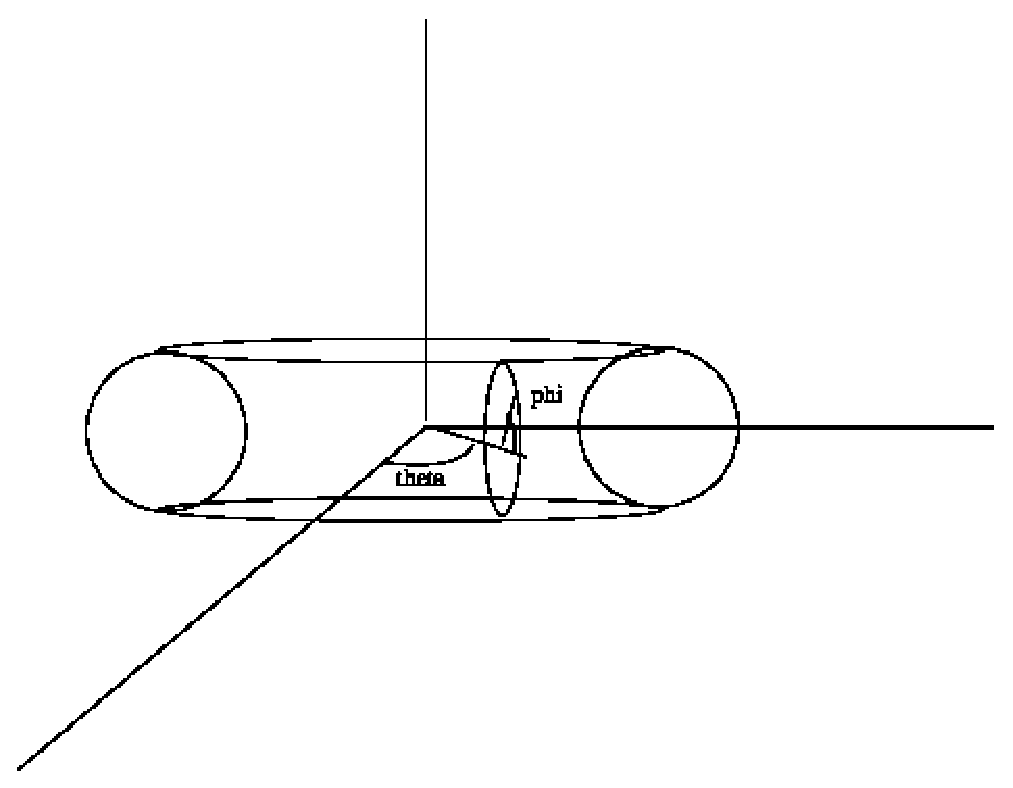
\includegraphics[scale=0.5]{images/img-mour-454}}
    \item \question{Montrer que $T$ est une surface régulière de $\Rr ^3$.}
\reponse{L'application $F$ est de classe $\mathcal{C}^\infty$ et injective.
 On calcule
 $X_\varphi=\begin{pmatrix}-\sin(\varphi)\cos(\theta)\\ -\sin(\varphi)\sin(\theta)\\ \cos (\varphi)\end{pmatrix}$
 et $X_\theta=\begin{pmatrix}-(2+\cos(\varphi))\sin(\theta)\\ (2+\cos(\varphi))\cos(\theta)\\ 0\end{pmatrix}$.
 Si $\varphi\not=0$, $\sin(\varphi)\not=0$ et les deux premières coordonnées sont indépendantes.
 Si $\varphi=0$, $X_\varphi=\begin{pmatrix}0\\0\\1\end{pmatrix}$ et $X_\theta=\begin{pmatrix}-\sin(\theta)\\ \cos(\theta)\\ 0\end{pmatrix}$
 sont indépendants.
 Ainsi, $dF$ est partout de rang $2$ donc un homéomorphisme local. Puisqu'elle est injective,
 l'application $F$ est donc un paramétrage.
 L'image $T$ est donc une surface régulière de $\Rr ^3$.}
    \item \question{Déterminer la courbure de Gauss $K$ de $T$ avec la métrique induite par le produit scalaire sur $\Rr ^3$,
c'est à dire la première forme fondamentale.(Expliquer d'abord votre démarche globale. Tout résultat
intermédiaire sera pris en compte).}
\reponse{On détermine d'abord la matrice de la première forme fondamentale
 $$G=\begin{pmatrix}
    1&0\\0&(2+\cos(\varphi))^2
   \end{pmatrix}$$
 On choisit comme champ de vecteurs normaux unitaires
 $$N=-\frac{X_\varphi\wedge X_\theta}{2+\cos(\varphi)}
 =\begin{pmatrix}\sin(\varphi)\cos(\theta)\\ \sin(\varphi)\sin(\theta)\\ -\cos (\varphi)\end{pmatrix}
 \wedge \begin{pmatrix}-\sin(\theta)\\ \cos(\theta)\\ 0\end{pmatrix}
 =\begin{pmatrix}
  \cos (\varphi)\cos(\theta)\\ \cos (\varphi)\sin(\theta)\\
 \sin(\varphi)
  \end{pmatrix}
 $$
 On détermine ensuite l'endomorphisme de Weingarten $W$ par 
 $$WX_\varphi=\frac{\partial N}{\partial \varphi}
 =\begin{pmatrix}
  -\sin (\varphi)\cos(\theta)\\ -\sin (\varphi)\sin(\theta)\\
 \cos(\varphi)\end{pmatrix}=X_\varphi$$
 $$\text{ et } \quad WX_\theta=\frac{\partial N}{\partial \theta}=
 \begin{pmatrix}
  -\cos (\varphi)\sin(\theta)\\ \cos (\varphi)\cos(\theta)\\0\end{pmatrix} =\frac{\cos(\varphi)}{2+\cos(\varphi)}X_\theta$$
 On en déduit que les valeurs propres de $W$ sont $1$ et $\frac{\cos(\varphi)}{2+\cos(\varphi)}$,
 et que la courbure de Gauss est donc $K(\varphi,\theta)=\frac{\cos(\varphi)}{2+\cos(\varphi)}$.}
    \item \question{Calculer $\int_T K(m)d\sigma(m)$.}
\reponse{\begin{eqnarray*}
  \int_T K(m)d\sigma(m)&=&\int_{]-\pi,\pi[\times ]-\pi,\pi[}K(\varphi,\theta)\sqrt{det G}d\varphi d\theta\\
 &=&\int_{]-\pi,\pi[\times ]-\pi,\pi[}\frac{\cos(\varphi)}{2+\cos(\varphi)} (2+\cos(\varphi))d\varphi d\theta\\
 &=&2\pi\int_{-\pi}^{\pi}\cos(\varphi)d\varphi=0.
  \end{eqnarray*}}
\end{enumerate}
}
